\section{Design and Implementation}\label{sec:implementation}

%%\PH{A detailed description of your parallel thread-pool based
%%  server. Point out the differences to the event-loop-based solution,
%%  and of course all the nice things like no locking etc.. What do you
%%  avoid wrt. the problem in traditional designs like dependencies, If
%%  possible, generalize the concepts from the Java-specific
%%  implementation. Are there any design/implementation specific
%%  alternatives that should be discussed. Also describe the example
%%  game and tell why this is a representative example in order to
%%  indicate that the results/conclusions are valid beyond the case
%%  study. \\ Screenshots?  Overview figure of the architecture? }

In our experimental prototype implementation of the LEARS concept, the
parallel approach is realized using thread pools and blocking queues.

\subsection{Thread pool}

Creation and deletion of threads incur large overheads,
and context switching is an expensive operation.  These overheads
constrain how a system can be designed, i.e., threads should be kept
as long as possible, and the number of threads should not grow
unbounded. We use a \textit{thread pool} pattern to work around these
constraints, and a thread pool executor (the Java
\texttt{ThreadPoolExecutor} class) to maintain the pool
of threads and a queue of tasks. When a thread is available, the
executor picks a task from the queue and executes it. The thread
pool system itself is not preemptive, so the thread runs each task
until it is done. This means that in contrast to normal threading,
each task should be as small as possible, i.e., larger units of work should
be split up into several sub-tasks.

The thread pool is a good way to balance the number of threads
when the work is split into extremely small units. When an active
element is created in the virtual world, it is scheduled for
execution by the thread pool executor, and the active element updates
its state exactly as in the single threaded case.
%
Furthermore, our thread pool supports the concept of delayed
execution. This means that tasks can be put into the work queue for
execution at a time specified in the future.
%
When the task is finished for one time slot, it can reschedule itself
for the next slot, delayed by a specified time. This allows active
elements to have any lifetime from one-shot executions to the duration
of the program. It also allows different elements to be updated at
different rates depending on the requirements of the game developer.

All work is executed by the same thread pool, including the slower I/O operations. This is a consistent and clear approach, but it does mean that game updates could be stuck waiting for I/O if there are not enough threads available. 

\subsection{Blocking queues}

The thread pool executor used as described above does not constrain
which tasks are executed in parallel. All systems elements
must therefore allow any of the other elements to execute concurrently. 

To enable a fast communication between threads with shared memory (and
caches), we use \textit{blocking queues}, using the Java
\texttt{Blocking\-Queue} class, which implements queues that are
synchronized separately at each end. This means that elements can be
removed from and added to the queue simultaneously, and since each of
these operations are extremely fast, the probability of blocking is
low. In the scenario analysed here, all active elements can potentially communicate with all others.
%
Thus, these queues allow information to be passed
between active objects. Each active object that can be influenced by
others has a blocking queue of messages. During its update, it  reads and processes
the pending messages from its queue. Messages are processed in the order they were put in the queue. Other active
elements put messages in the queue to be processed when they need to
change the state of other elements in the game.

Messages in the queues can only contain relative information, and not absolute values. This restriction ensures that the change is always based on updated data. For example, if a projectile needs to tell a player character that it took damage, it should only inform the player character about the amount of damage, not the new health total. Since all changes are put in the queue, and the entire queue is processed by the same work unit, all updates are based on up-to-date data.
%This form of communication is extremely fast. As all threads share the
%same memory, trasfer through memory. Data can even be transfered
%without leaving cache.
\subsection{Our implementation}
% Also describe the example
% game and tell why this is a representative example in order to
% indicate that the results/conclusions are valid beyond the case
% study.
 
To demonstrate LEARS, we have implemented a prototype
game containing all the basic elements of a full MMOG with the
exception of persistent state. The basic architecture of the
game server is described in figure~\ref{fig:server}. The thread 
pool size can be configured, and will execute the different workloads 
on the CPU cores. The workloads include processing of network messages, moving computer controlled elements (in this prototype only projectiles) checking for collisions and hits and sending outgoing network messages.
%
%\HKS{Kjetil: Kan du kort beskrive de forskjellige workloadene som serveren
%eksekverer i thread pool her?}

Persistent state do introduce some complications, but as database
transactions are often not time critical and can usually be scheduled
outside peak load situations, we leave this to future work.

\begin{figure}
\centering
%\vspace{-3mm}
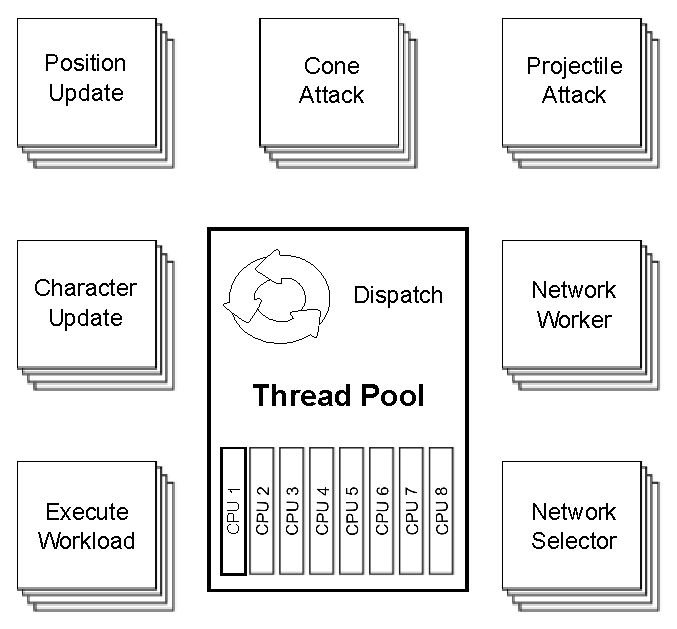
\psfig{file=FIG/server.eps,width=\columnwidth}
\vspace{-3mm}
\caption{Design of the Game Server}
\vspace{-3mm}
\label{fig:server}
\end{figure}

\begin{figure}
  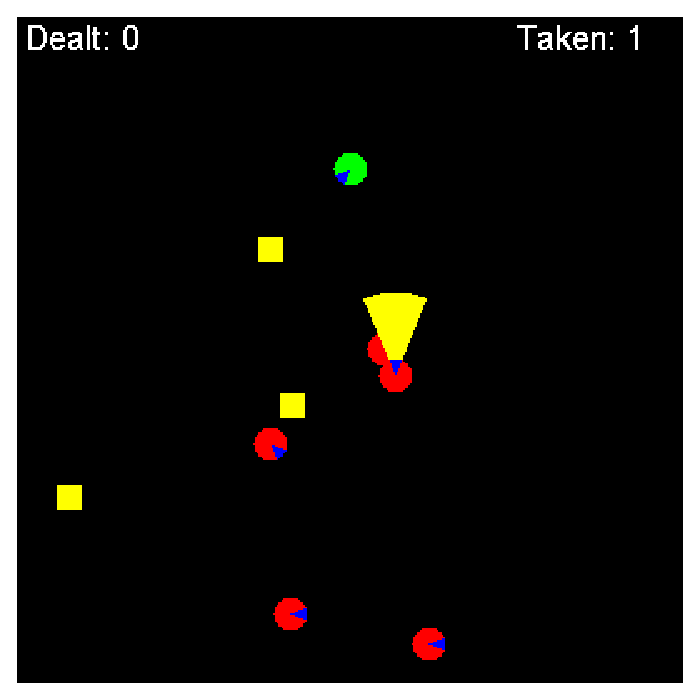
\includegraphics[width=\columnwidth]{FIG/screenshot}
  \caption{Screen shot of a game with six players.}
  \label{fig:screen}
\end{figure}
In the game, each player controls a small circle ("the
character") with an indicator for which direction they are heading
(see figure~\ref{fig:screen}). The
characters are moved around by pressing keyboard buttons. They also
have two types of attack, i.e.,  one projectile and one instant area of effect
attack. Both attacks are aimed straight ahead. If an attack hits
another player character, the attacker gets a positive point, and the
character that was hit gets a negative point. The game
provides examples of all the elements of the design described
above:
\begin{itemize}
\item The player character is a long lifetime active object. It
  processes messages from clients, updates states and potentially
  produces other active objects (attacks). In addition to position,
  which all objects have, the player also has information about how
  many times it has been hit and how many times it has hit others. The
  player character also has a message queue to receive messages from
  other active objects. At the end of its update, it enqueues
  itself for the next update unless the client it represents has
  disconnected.
\item The frontal cone attack is a one shot task that finds player
  characters in its designated area and sends messages to those hit so
  they can update their counters, as well as back to the attacking
  player informing about how many were hit.
\item The projectile is a short lifetime object that moves in the
  world, checks if it has hit anything and reschedules itself for
  another update, unless it has hit something or ran to the end of its
  range. The projectile can only hit one target.
\end{itemize}

%\begin{figure}[h]
%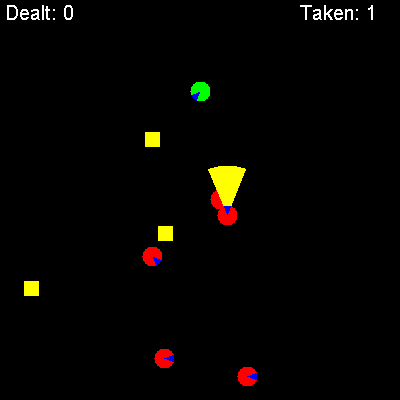
\includegraphics[width=1.0\linewidth, bb=0 0 400 400]{FIG/screenshot.png}
%\caption{Screenshot of the game with six players.}
%\end{figure}

%% \begin{figure}
%% \centering
%% %\vspace{-3mm}
%% 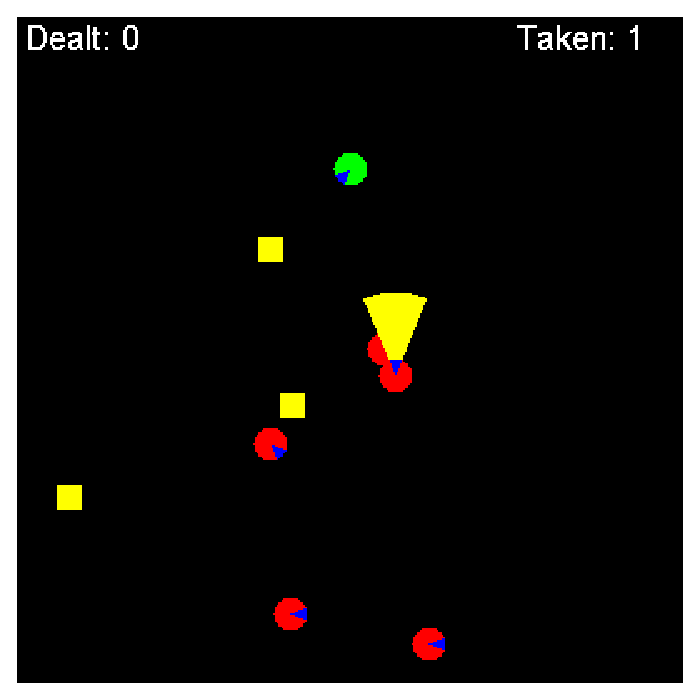
\psfig{file=FIG/screenshot.eps,width=4cm}
%% \vspace{-3mm}
%% \caption{Screenshot of game with six players.}
%% \vspace{-3mm}
%% \label{fig:screen}
%% \end{figure}

To simulate an MMORPG workload that grow linearly with number of
players, especially collision checks with the ground and other static
objects, we have included a synthetic load which emulates collision
detection with a high-resolution terrain mesh. The synthetic load
ensures that the cache is regularly flushed
%an array of floating
%point values represents a part of the gameworld. For each scheduled
%update, each character has to perform a square operation on a given
%number of elements in the array. The operation is seeded with a
%randomly generated value in order to avoid runtime optimizations in
%the virtual machine. Which elements are processed depends on the
%player's position in the gameworld. How many array elements are
%processed determines the severity of the load. By adding the synthetic
%load, the cache is dirtied 
to enhance the realism of our game server prototype compared to a
large-scale game server.
%For our experiments, 1000
%array elements were processed for each character update, emulating
%collision detection with a high-resolution terrain mesh.

The game used in these experiments is simple, but it contains examples of all elements typically available in the action based parts of a typical MMO-like game. 

The system described in this paper is implemented in Java. This
programming language has strong support for multi-threading and has
well-tested implementations of all the required components. The
absolute values resulting from these experiments depend strongly on
the complexity of the game, as a more complex game would require more
processing. In addition, the absolute values depend on the runtime
environment, especially the server hardware, and the choice of programming
language also influence absolute results from the
experiments. However, the focus of this paper is the relative results,
as we are interested in comparing scalability of the multi-threaded
solution with a single-threaded approach and whether the
multi-threaded implementation can handle the quadratic increase in
traffic as new players join.
